
\documentclass{beamer}


\mode<presentation>
{
  \usetheme{Boadilla}


  \setbeamercovered{transparent}
}


\usepackage{cmap}					% поиск в PDF
\usepackage[T2A]{fontenc}			% кодировка
\usepackage[utf8]{inputenc}			% кодировка исходного текста
\usepackage[english,russian]{babel}	% локализация и переносы
\usepackage{mathtext}
\usepackage{times}
\usepackage{subfigure}

% title
\title[Triple crystal difractometry] % (optional, use only with long paper titles)
{Трехкристальная рентгеновская дифрактометрия}


\author[Atknin, Chukhovsky, Marchenkov ] 
{I.~Atknin\inst{1,2,3} \and F.~Chukhovsky\inst{2} \and N.~Marchenkov\inst{2,3}}


\institute[] % (optional, but mostly needed)
{
  \inst{1}%
  Department of optics, spectroskopy and physics of nanosystems\\
  Moscow State University
  \and
  \inst{2}%
X-ray analysis technique and
synchrotron radiation laboratory\\
 Shubnikov Institute of Crystallography, Russian Academy of Sciences.
  \and
  \inst{3}%
  National Research Centre "Kurchatov Institute"\\
 Department of Nano-, Bio-, Info-, and Cognitive Sciences and Technologies}
\date[\today ] % (optional)

\begin{document}

% page#1
\begin{frame}
  \titlepage
\end{frame}


% page#2
\begin{frame}{qz and qy [1]}
\begin{figure}[h] 
   \centering
   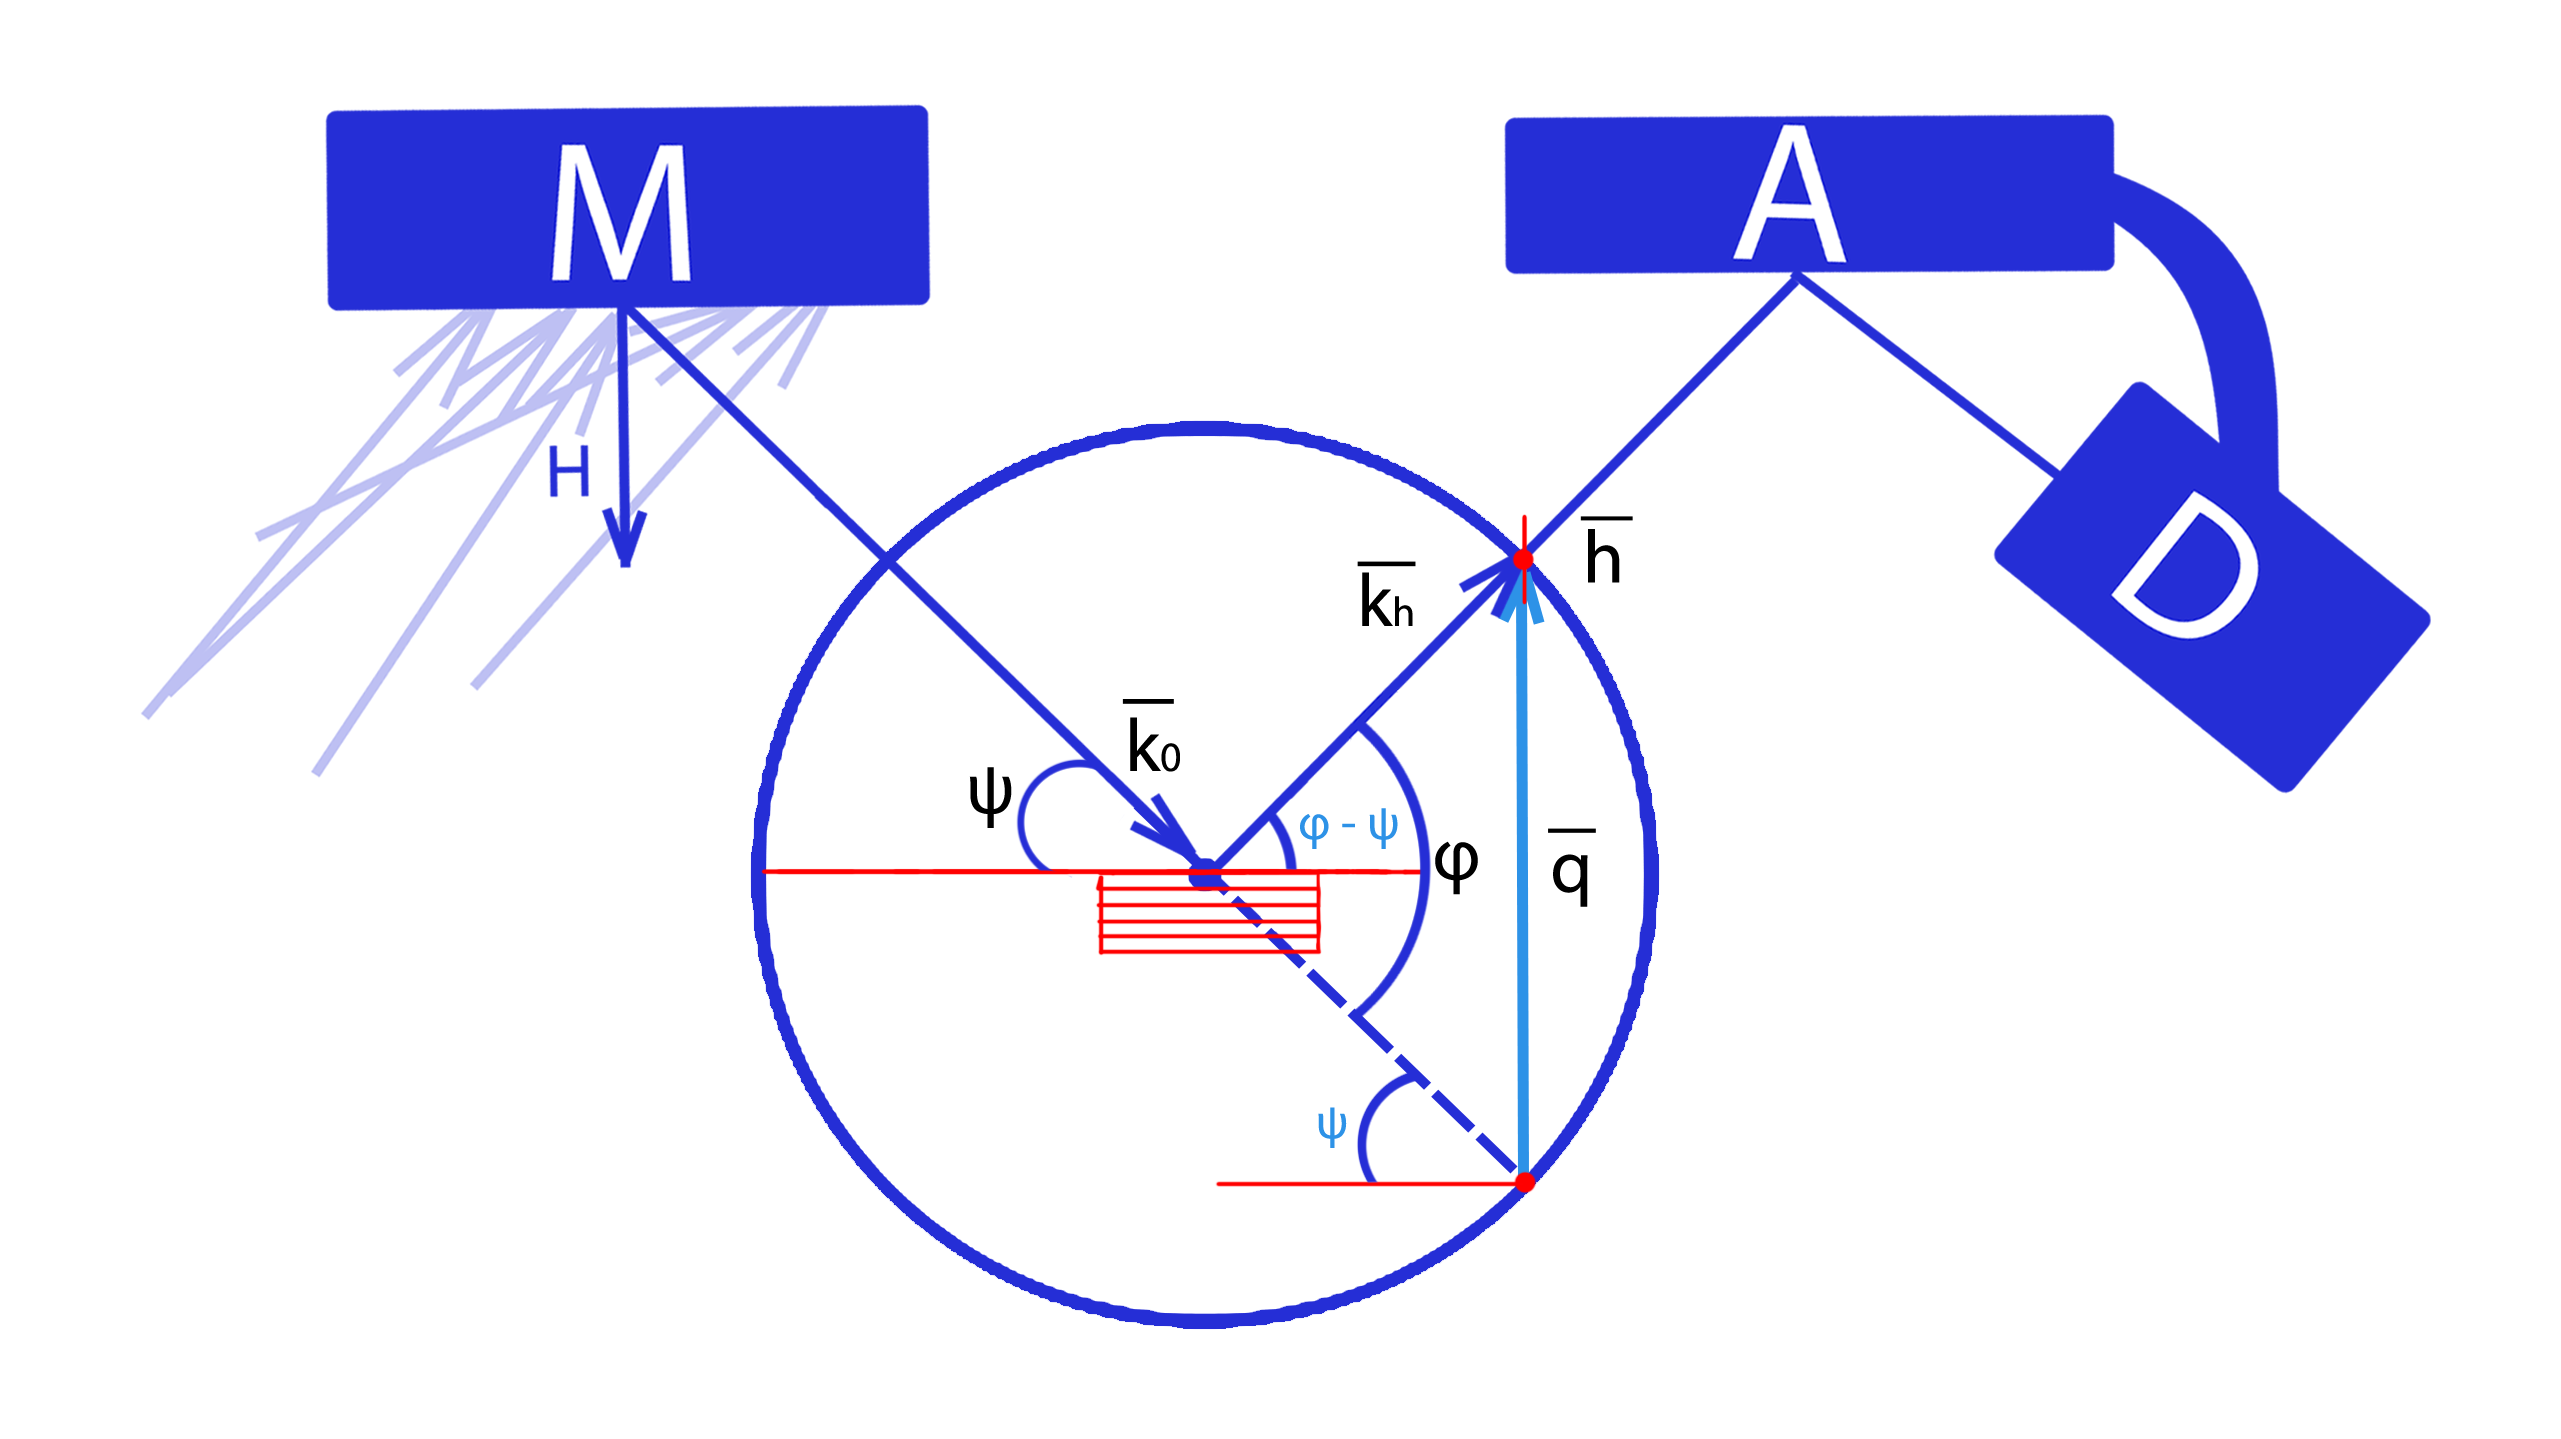
\includegraphics[width=2.5in]{graph/ewald_general.png} 
   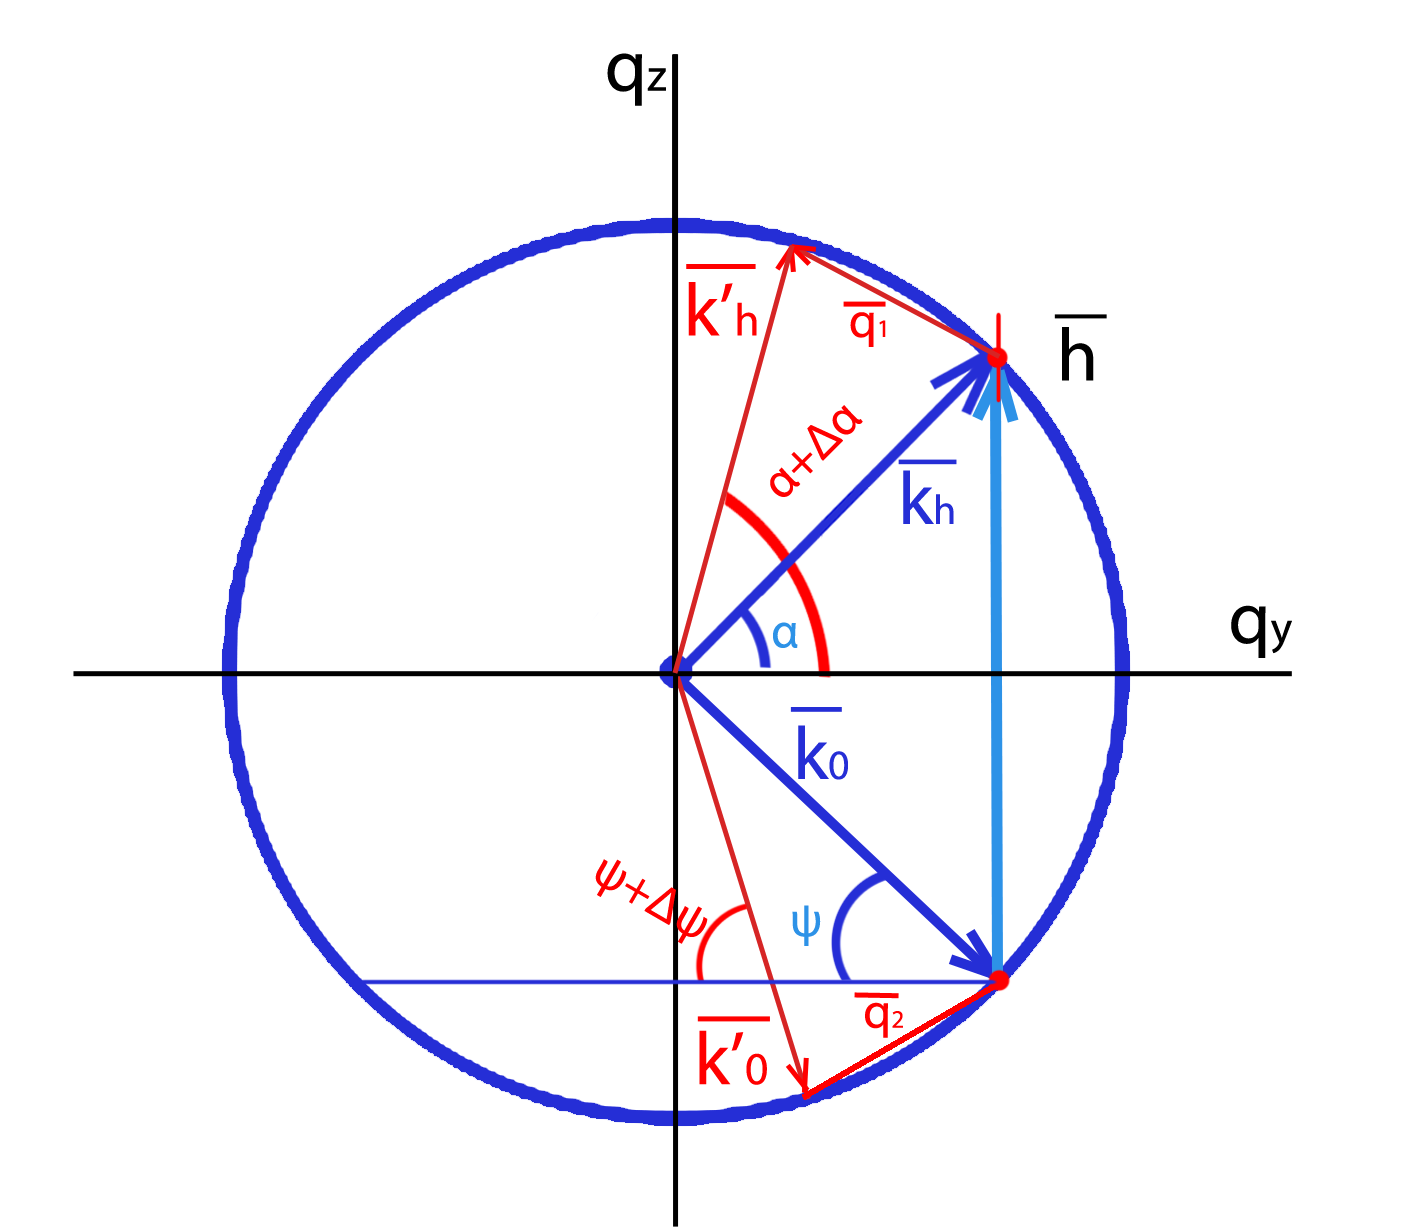
\includegraphics[width=2.0in]{graph/ewald_help.png} 
   \label{default}
\end{figure}
$\pmb q$ - the deviation of the scattering vector,
$h$ - the reciprocal lattice point.
The left figure – illustrates the case when the specimen angle, \fbox{$\psi$}, and the analyser angle, \fbox{$\phi$}, are set so as to satisfy the Bragg condition.
\end{frame}


% page#2
\begin{frame}{qz and qy  [1]}
$q_1:$
\begin{alignat}{2}
\frac{q_y}{|k|} = cos\alpha -  cos(\alpha - \Delta \alpha) \\
\frac{q_z}{|k|} = sin(\alpha + \Delta \alpha) -  sin\alpha 
\end{alignat}
$q_2:$
\begin{alignat}{2}
\frac{q_y}{|k|} = cos\psi -  cos(\psi - \Delta \psi) \\
\frac{q_z}{|k|} = sin(\psi + \Delta \psi) -  sin\psi 
\end{alignat}
where:
$$ sin(a + b) = sin (a) \cdot cos (b)  - sin (b)  \cdot cos (a)  $$
$$ cos(a + b) = cos (a) \cdot cos (b)  - sin (b)  \cdot sin (a)  $$
$$cos  \Delta \alpha  = cos \Delta \psi = 1 $$
$$sin  \Delta \alpha  = \Delta \alpha $$
$$sin \Delta \psi =  \Delta \psi$$
\end{frame}


% page#2
\begin{frame}{qz and qy  [1]}

\begin{alignat}{2}
\frac{q_{1y}+q_{2y}}{|k|} =\frac{q_y}{\pmb  k} =-\Delta \alpha \cdot sin\alpha + \Delta \psi \cdot sin \psi \\
\frac{q_{1z}+q_{2z}}{|k|} =\frac{q_z}{\pmb  k} = \Delta \alpha \cdot cos\alpha +   \Delta \psi \cdot cos \psi 
\end{alignat}
where
 $$\alpha = \phi - \psi$$
$$\Delta \alpha = \Delta\phi - \Delta\psi$$
for the result we have
\begin{alignat}{2}
\frac{q_y}{| k|} =\Delta \psi \cdot sin \psi - (\Delta \phi - \Delta \psi) \cdot sin(\phi - \psi) \\
\frac{q_z}{|k|} =\Delta \psi \cdot cos \psi + (\Delta \phi - \Delta \psi) \cdot cos(\phi - \psi)   
\end{alignat}
for symmetric reflection:
$$\psi = \theta_B$$
$$\phi - \psi= \theta_B$$

\end{frame}

% page#3 
\begin{frame}{$\theta-2\theta$ scan. Separation of lattice tilts and \fbox{strains}}
Any region of the specimen which also has lattice
parameter \fbox d but is tilted with respect to the original region will never provide
scattering which reaches the detector;
\begin{figure}[h] 
\centering
\includegraphics[height=1.2in]{graph/animation/1_1.jpg} 
\includegraphics[height=1.1in]{graph/animation/1_2.jpg} 
\end{figure}
However, another region of the sample with lattice parameter \fbox d may come to a position where the Bragg angle is satisfied.
\end{frame}

\begin{frame}{$\theta-2\theta$ scan. Separation of lattice tilts and \fbox{strains}}
Any region of the specimen which also has lattice
parameter \fbox d but is tilted with respect to the original region will never provide
scattering which reaches the detector;
\begin{figure}[h] 
\centering
\includegraphics[height=1.2in]{graph/animation/2_1.jpg} 
\includegraphics[height=1.1in]{graph/animation/2_2.jpg} 
\end{figure}
However, another region of the sample with lattice parameter \fbox d may come to a position where the Bragg angle is satisfied.
\end{frame}

\begin{frame}{$\theta-2\theta$ scan. Separation of lattice tilts and \fbox{strains}}
Any region of the specimen which also has lattice
parameter \fbox d but is tilted with respect to the original region will never provide
scattering which reaches the detector;
\begin{figure}[h] 
\centering
\includegraphics[height=1.2in]{graph/animation/3_1.jpg} 
\includegraphics[height=1.1in]{graph/animation/3_2.jpg} 
\end{figure}
However, another region of the sample with lattice parameter \fbox d may come to a position where the Bragg angle is satisfied.
\end{frame}

\begin{frame}{$\theta-2\theta$ scan. Separation of lattice tilts and \fbox{strains}}
Any region of the specimen which also has lattice
parameter {\bfseries{d}} but is tilted with respect to the original region will never provide
scattering which reaches the detector;
\begin{figure}[h] 
\centering
\includegraphics[height=1.2in]{graph/animation/4_1.jpg} 
\includegraphics[height=1.1in]{graph/animation/4_2.jpg} 
\end{figure}
However, another region of the sample with lattice parameter \fbox d may come to a position where the Bragg angle is s§tisfied.
\end{frame}

\begin{frame}{$\theta-2\theta$ scan. Separation of lattice tilts and \fbox{strains}}
Any region of the specimen which also has lattice
parameter \fbox d but is tilted with respect to the original region will never provide
scattering which reaches the detector;
\begin{figure}[h] 
\centering
\includegraphics[height=1.2in]{graph/animation/5_1.jpg} 
\includegraphics[height=1.1in]{graph/animation/5_2.jpg} 
\end{figure}
However, another region of the sample with lattice parameter \fbox d may come to a position where the Bragg angle is satisfied.
\end{frame}

% page 4
\begin{frame}{A scattering map in reciprocal space.}
\begin{figure}[h] 
\centering
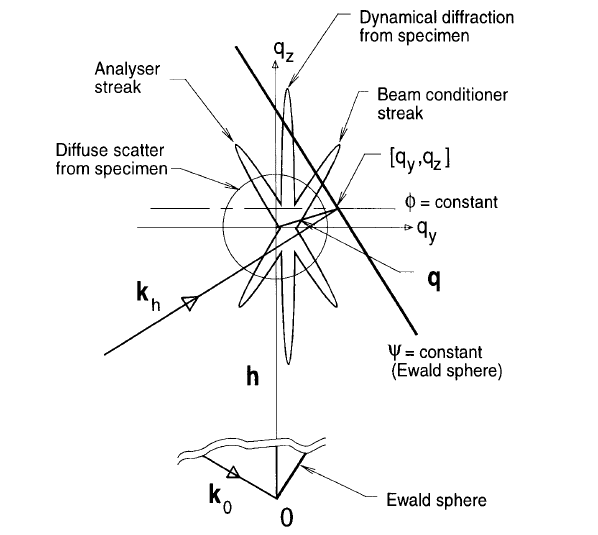
\includegraphics[height=4in]{graph/qxqz.png} 
\end{figure}
dsf
\end{frame}


% page 5
\begin{frame}{Total intensity}
\begin{alignat}{2}
I(\varepsilon, \omega,\Delta \theta_1) = 	\int\limits_{-\infty}^\infty R_1 (\Delta \theta_1)
R_2(\Delta \theta_1+\omega)R_3(\Delta \theta_1+2\omega - \varepsilon)\cdot \pmb{d}\Delta \theta_1
\end{alignat}
\begin{figure}[t] 
\centering
\includegraphics[width=5in]{graph/trd.png} 
\end{figure}
\end{frame}



% page 5
\begin{frame}{CASE A \fbox{$|\omega| \gg \Delta \theta_B $ }}
where, $\Delta \theta_B $ - full width at half maximum, abbreviated as FWHM\\
\begin{itemize}
\item $\Delta \theta_1 = 0$ – the condition for maximum intensity from the monochromator  \\ 
$$I(\varepsilon,\omega, 0) = \int\limits_{-\infty}^\infty R_1 (0)
R_2(\omega)R_3(2\omega - \varepsilon) \cdot \pmb{d}\Delta\theta_1$$ \\
Maximum intensity for the specimen is $\varepsilon = 2 \omega$ (take in to account the condition $|\omega| \gg \Delta \theta_B $) - \fbox{MAIN PEAK (MP)}
$$I_{MP}^{max} = R_1(0)R_2(\omega)R_3(0)\cdot \pmb{d}\Delta\theta_1$$\\
The MP intensity is defined by the intensity $R_2(\omega)$ on the ROCKING CURVE tail for the specimen
\end{itemize}
\end{frame}


%page6
\begin{frame}{CASE A \fbox{$|\omega| \gg \Delta \theta_B $ }}
\begin{itemize}
\item  $\Delta \theta_1 = -\omega$  - the condition for maximum intensity from the specimen \\
c
Maximum intensity is $\varepsilon = \omega$ - \fbox{PSEUDO-PEAK (PP) or MONOCHROMATOR PSEUDO-PEAK}
$$I_{PPM}^{max} = R_1(-\omega)R_2(0)R_3(0)\cdot \pmb{d}\Delta\theta_1$$\\
The PP intensity is defined by the intensity $R_1(-\omega)$ on the ROCKING CURVE tail for the monochromator
\end{itemize}
\end{frame}



%page7
\begin{frame}{CASE B \fbox{$|\varepsilon| \gg \Delta \theta_B $ }}
\begin{itemize}
\item  $\Delta \theta_1 = 0$\\
$$I(\varepsilon, \omega, 0) = \int\limits_{-\infty}^\infty R_1(0)
R_2(\omega)R_3(2\omega - \varepsilon) \cdot \pmb{d}\Delta\theta_1$$ \\
There are two conditiond to have maximima 
\begin{itemize}
\item $\omega=0$ - $R_3(-\varepsilon)$ \fbox{ANALYSER PSEUDO-PEAK} - realize on the ROCKING CURVE tail for the analyser \\
$$I_{PPA}= R_1(0)R_2(0)R_3(-\varepsilon)\cdot \pmb{d}\Delta\theta_1$$\\
\item $\omega = \varepsilon/2$ \fbox{MAIN PEAK}
$$I_{PPA}= R_1(0)R_2(\varepsilon/2)R_3(0)\cdot \pmb{d}\Delta\theta_1$$
\end {itemize}
\end{itemize}
\end{frame}

%page8
\begin{frame}{CASE B \fbox{$|\varepsilon| \gg \Delta \theta_B $ }}
\begin{itemize}
\item  $\Delta \theta = -\varepsilon$
$$I_{PPM}= R_1(-\varepsilon)R_2(\omega - \varepsilon)R_3(2\omega - 2\varepsilon)\cdot \pmb{d}\Delta\theta_1$$ \\ the condition for maximum intensity $\omega = \varepsilon$\\
The pseudo-peak is defined by the intensity on the ROCKING CURVE tail for the monochromator
$$I_{PPM}^{max} = R_1(-\varepsilon)R_2(0)R_3(0)\cdot \pmb{d}\Delta\theta_1$$
\end{itemize}
\end{frame}


%page9
\begin{frame}{CASE C $\theta/2\theta$ - scan \fbox{$\varepsilon = 2\omega $ }}

\end{frame}


\begin{frame}{incipient questions}
Here I will ask you for some questions.
\end{frame}

\begin{frame}{References}

[1] Bowen D.K., Tanner B.K. High resolution X-ray Diffractometry and Topography p.169
\end{frame}
\end{document}


